\def\dlt{0.4}
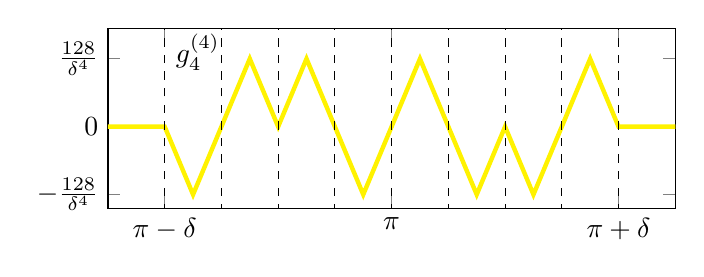
\begin{tikzpicture}
\begin{axis}[
    width=250pt,height=110pt,
    xmin=pi-0.5,xmax=pi+0.5,
    ymin=-1.2,ymax=1.45,
    samples=50,
    xtick={pi-\dlt, pi, pi+\dlt},
    xticklabels={$\pi - \delta$, $\pi$, $\pi + \delta$},
    ytick={-1, 0, 1},
    yticklabels={$-\frac{128}{\delta^4}$, $0$, $\frac{128}{\delta^4}$},
    grid style={line width=.1pt, draw=gray!10}]

    \addplot[yellow, ultra thick] coordinates {
        (0, 0) (pi-\dlt, 0) (pi-7*\dlt/8, -1) (pi-5*\dlt/8, 1) (pi-\dlt/2, 0) (pi-3*\dlt/8, 1) (pi-\dlt/8, -1) (pi+\dlt/8, 1) (pi+3*\dlt/8, -1) (pi+\dlt/2, 0) (pi+5*\dlt/8, -1) (pi+7*\dlt/8, 1) (pi+\dlt, 0) (4,0)
    };

    \draw [dashed] (axis cs:{pi-\dlt},-2) -- (axis cs:{pi-\dlt},2);
    \draw [dashed] (axis cs:{pi-3*\dlt/4},-2) -- (axis cs:{pi-3*\dlt/4},2);
    \draw [dashed] (axis cs:{pi-\dlt/2},-2) -- (axis cs:{pi-\dlt/2},2);
    \draw [dashed] (axis cs:{pi-\dlt/4},-2) -- (axis cs:{pi-\dlt/4},2);
    \draw [dashed] (axis cs:{pi},-2) -- (axis cs:{pi},2);
    \draw [dashed] (axis cs:{pi+\dlt/4},-2) -- (axis cs:{pi+\dlt/4},2);
    \draw [dashed] (axis cs:{pi+\dlt/2},-2) -- (axis cs:{pi+\dlt/2},2);
    \draw [dashed] (axis cs:{pi+3*\dlt/4},-2) -- (axis cs:{pi+3*\dlt/4},2);
    \draw [dashed] (axis cs:{pi+\dlt},-2) -- (axis cs:{pi+\dlt},2);
    
    \node at (axis cs:2.8,1.1) {$g^{(4)}_4$};
\end{axis}
\end{tikzpicture}
\undef\dlt